\section{Etape C : génération de code}
L'étape C met en coopération les paquetages suivants :

\begin{center}
  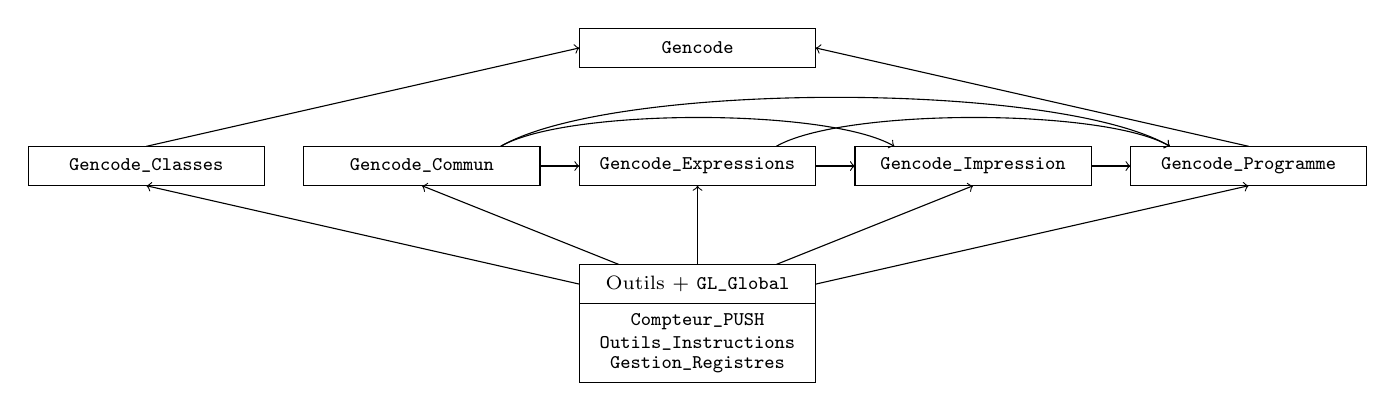
\begin{tikzpicture}[scale=0.5,font=\scriptsize]
    \draw (14,0) rectangle (20,3);
    \draw (17,0) node[above] {\verb!Gestion_Registres!};
    \draw (17,1) node {\verb!Outils_Instructions!};
    \draw (17,2) node[below] {\verb!Compteur_PUSH!};
    \draw (14,2) -- (20,2);
    \draw (17,2.5) node {Outils + \verb!GL_Global!};


    \draw (0,5) rectangle (6,6);
    \draw (3,5.5) node {\verb!Gencode_Classes!};
    \draw[->] (3,6) -- (14,8.5);
    \draw[<-] (3,5) -- (14,2.5);


    \draw (7,5) rectangle (13,6);
    \draw (10,5.5) node {\verb!Gencode_Commun!};
    \draw[<-] (10,5) -- (15,3);
    \draw[->] (12,6) to[bend left, looseness=0.5] (29,6);
    \draw[->] (12,6) to[bend left, looseness=0.5] (22,6);

    \draw[->] (13,5.5) -- (14,5.5);

    \draw (14,5) rectangle (20,6);
    \draw (17,5.5) node {\verb!Gencode_Expressions!};
    \draw[<-] (17,5) -- (17,3);
    \draw[->] (19,6) to[bend left, looseness=0.5] (29,6);

    \draw[->] (20,5.5) -- (21,5.5);

    \draw (21,5) rectangle (27,6);
    \draw (24,5.5) node {\verb!Gencode_Impression!};
    \draw[<-] (24,5) -- (19,3);

    \draw[->] (27,5.5) -- (28,5.5);

    \draw (28,5) rectangle (34,6);
    \draw (31,5.5) node {\verb!Gencode_Programme!};
    \draw[->] (31,6) -- (20,8.5);
    \draw[<-] (31,5) -- (20,2.5);


    \draw (14,8) rectangle (20,9);
    \draw (17,8.5) node {\verb!Gencode!};
  \end{tikzpicture}
\end{center}


\begin{description}
\item[Outils\_Instructions] : paquetage responsable de la construction du programme assembleur, sous la forme d'un chaînage de lignes.

  Ce paquetage permet basiquement d'insérer une nouvelle ligne en fin de code ou d'afficher le programme ainsi construit. Cependant, il s'est vu ajouté les fonctionnalités suivantes :

  \begin{itemize}
  \item centralisation du booléen \verb!Check!, indiquant s'il faut écrire les vérifications de débordement.
  \item inclusion de la séquence \verb!TSTO!, \verb!BOV!, \verb!ADDSP! en début de chaque bloc (ie. programme principal, corps de méthode ou code d'initialisation des champs d'une classe), mise à jour de leurs opérandes lorsque les informations nécessaires deviennent disponibles et ajout éventuel du \verb!SUBSP! en fin de bloc.
  \item insertion de code en début de bloc (utilisé pour la séquence de sauvegarde des registres)
  \end{itemize}

  Ce paquetage permet donc de centraliser et d'abstraire toutes les opérations affectant le chaînage des instructions.

\item[Gestion\_Registres] : paquetage responsable de l'allocation des registres
  
  Son fonctionnement étant complexe, il sera détaillé en section \ref{registres} (page \pageref{registres}).
  
\item[Compteur\_PUSH] : paquetage servant à retenir la place totale utilisée dans la pile pour le bloc courant.
  
  Son fonctionnement est assez simple : chaque incrémentation du sommet de pile (\verb!ADDSP! ou \verb!PUSH!) doit s'accompagne d'un appel à la procédure \verb!Compte_PUSH!. De même, tout appel à \verb!SUBSP! ou \verb!POP! doit s'accompagner d'un appel à \verb!Compte_POP!. Ces deux primitives permettent de maintenir un compteur interne, ainsi que la valeur maximale atteinte par celui-ci depuis le début du bloc.

        Ainsi, en fin d'évaluation du bloc, on peut connaître la place totale nécessaire pour toute l'évaluation de celui-ci (et donc en informer le paquetage \verb!Outils_Instructions! pour mettre à jour les opérandes de \verb!TSTO! et \verb!ADDSP!).
        
      \item[Gencode\_Classes] : paquetage responsable de la passe 1.

        Construit la tables des méthodes et place, dans chaque \verb!Noeud_Classe!, l'opérande contenant l'adresse de la table des méthodes associée.
      \item[Gencode\_Commun] : ensemble des primitives communes à la passe 2.

        Ce paquetage contient notamment :
        \begin{itemize}
        \item Un compteur global pour éviter la répétition des étiquettes
        \item La procédure commune de mise au point (\verb!Mettre_Au_Point!)
        \item Les procédure de création de la méthode \verb!Object.equals! et de la gestion des messages d'erreur
        \item La fonction \verb!Assure_Registre!, qui sera détaillée par la suite
        \end{itemize}

      \item[Gencode\_Expressions] : paquetage responsable de l'évaluation des sous-arbres d'expression.
      \item[Gencode\_Impression] : paquetage responsable de l'impression des données (\verb!print! et \verb!println!).
      \item[Gencode\_Programme] : point d'entrée de la passe 2.

        Ce paquetage gère notamment :
        \begin{itemize}
        \item le parcours des blocs d'instructions (programme principal et corps des méthodes)
        \item les déclarations (de variables et de champs)
        \item l'initialisation des champs
        \item les structures de contrôle (\verb!if! et \verb!while!)
        \end{itemize}

        Il s'agit donc du lien entre tous les paquetages de la passe 2 (\verb!Gencode_Commun!, \verb!Gencode_Expressions! et \verb!Gencode_Impression!).

      \item[Gencode] : point d'entrée de la génération de code.

        Ce paquetage se charge d'initialiser les différents paquetage et de lancer les passes 1 et 2.
\end{description}

\subsection{Passe 1 : construction des tables des méthodes (paquetage \texttt{Gencode\_Classes})}
On distingue 2 sous étapes : 
\begin{itemize}
\item Construction du tableau des étiquettes des méthodes
\item Génération du code pour construire les tables des méthodes
\end{itemize}

Les tables des méthodes sont construites progressivement lors du parcours des classes. Les raisons d'un tel choix seront précisées plus loin.

\subsubsection{Construction du tableau des étiquettes des méthodes}
Afin de pouvoir construire la table des méthodes, il est nécessaire de connaître le nombre de méthodes, leur nom ainsi que l'adresse de la table des méthodes de la super-classe. C'est pourquoi la structure suivante est utilisée :

\begin{center}
  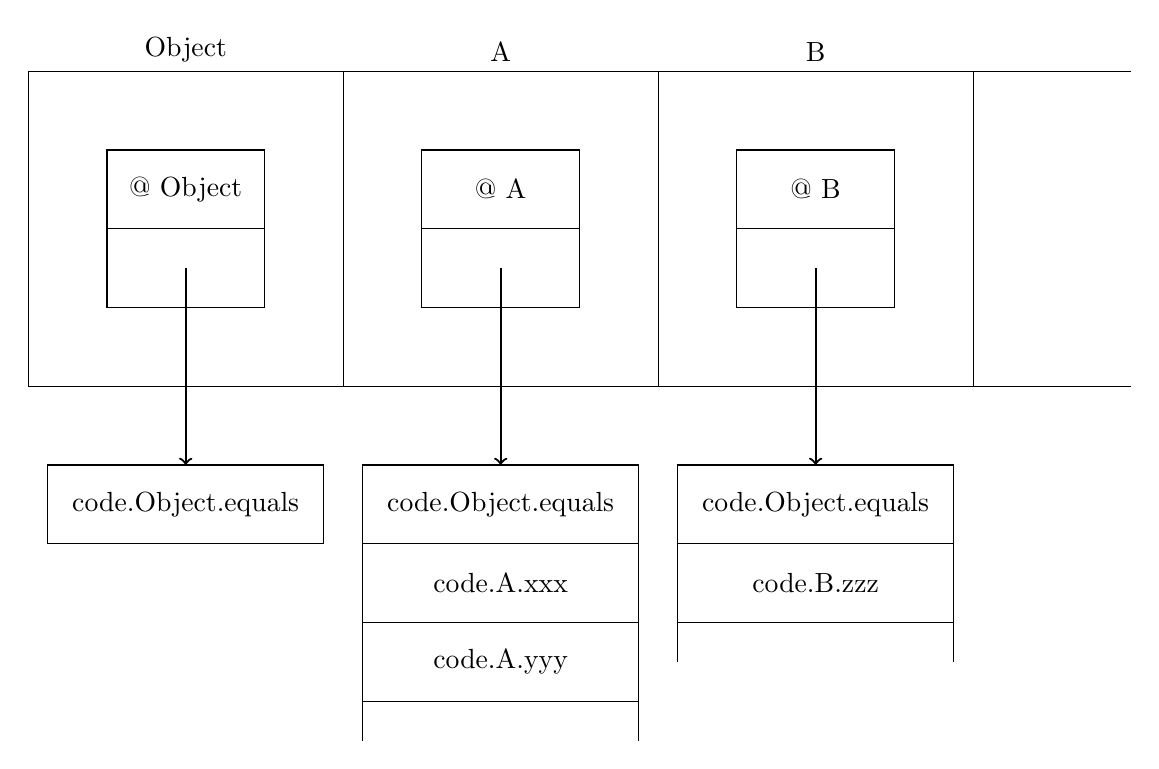
\begin{tikzpicture}
    \draw (0,0) grid[step=4,thick] (14,4);

    \draw (2,4) node[above] {Object};
    \draw (1,1) rectangle (3,3);
    \draw (1,2) -- (3,2);
    \draw (2,2.5) node {@ Object};
    \draw [->,thick] (2,1.5) -- (2,-1);
    
    \draw (0.25,-2) rectangle (3.75,-1);
    \draw (2,-1.5) node {code.Object.equals};

    \draw (6,4) node[above] {A};
    \draw (5,1) rectangle (7,3);
    \draw (5,2) -- (7,2);
    \draw (6,2.5) node {@ A};
    \draw [->,thick] (6,1.5) -- (6,-1);

    \draw (4.25,-4.5) -- (4.25,-1) -- (7.75,-1) -- (7.75,-4.5);
    \draw (6,-1.5) node {code.Object.equals};
    \draw (4.25,-2) -- (7.75,-2);
    \draw (6,-2.5) node {code.A.xxx};
    \draw (4.25,-3) -- (7.75,-3);
    \draw (6,-3.5) node {code.A.yyy};
    \draw (4.25,-4) -- (7.75,-4);

    \draw (10,4) node[above] {B};
    \draw (9,1) rectangle (11,3);
    \draw (9,2) -- (11,2);
    \draw (10,2.5) node {@ B};
    \draw [->,thick] (10,1.5) -- (10,-1);

    \draw (8.25,-3.5) -- (8.25,-1) -- (11.75,-1) -- (11.75,-3.5);
    \draw (10,-1.5) node {code.Object.equals};
    \draw (8.25,-2) -- (11.75,-2);
    \draw (10,-2.5) node {code.B.zzz};
    \draw (8.25,-3) -- (11.75,-3);
    
  \end{tikzpicture}
\end{center}


Cette structure est remplie grâce à une passe dans l'arbre, qui utilise les décors des \verb!Noeud_Ident! afin de récupérer les informations nécessaires (nom de la super classe, nombre de méthodes, numéro de chaque méthode ...). 

Le tableau est géré par le package \verb!Tables!. Cependant, l'ordre de déclaration des classes est important pour construire une table des méthodes cohérente.
Le tableau est donc construit progressivement, afin de ne pas devoir le re-parcourir par la suite.

\subsubsection{Construction de la table des méthodes}

Pour chaque classe, la structure obtenue dans la page précédente ainsi que l'adresse de la super classe sont retournées afin de pouvoir construire la table des méthodes.
Une simple lecture des informations reçues permet, à l'aide des instructions \verb!LEA!, \verb!LOAD! et \verb!STORE!, de générer le code construisant la table des méthodes.

\subsection{Passe 2 : génération du code}
La structure principale de la génération de code est un parcours de l'arbre décoré par l'étape B.
Ce parcours est effectué par les paquetages \verb!Gencode_Expression!, \verb!Gencode_Impression! et \verb!Gencode_Programme!, chacun étant responsable du parcours d'un sous-arbre spécifique.
Ces trois paquetages sont structurés de la même manière, et possèdent chacun :
\begin{itemize}
\item un point d'entrée
\item un ensemble de procédures (ou fonctions) possédant des prototypes similaires
\end{itemize}

\subsubsection{Les expressions (paquetage \texttt{Gencode\_Expressions})}

Pour évaluer les expressions, on utilise des fonctions de la forme :
\begin{verbatim}
  function Place_Xxx (A : in Arbre, ...) return Operande
\end{verbatim}
Ce type de fonction doit se charger d'évaluer le sous-arbre \verb!A! et de retourner l'emplacement du résultat.
Dans le cas où l'emplacement retourné est un registre, une telle fonction se comporte exactement comme la fonction \verb!Allouer! : seul le registre retourné et celui précédemment alloué peuvent être utilisés (soit \verb!RA! et \verb!RB!, voir section \ref{registres}, page \pageref{registres}).

Dans le cas d'un opérateur binaire, le corps de la fonction \verb!Place_Op_Binaire! pourrait être de forme :
\begin{enumerate}
\item Calculer l'opérande gauche (alloue un registre)
\item Cacluler l'opérande droite (alloue un autre registre)
\item Effectuer l'opération et placer le résultat dans le premier registre.

  On peut effectuer ce calcul car l'allocation de l'opérande droite autorise l'utilisation du registre précédemment alloué, c'est à dire l'opérande gauche.
\item Libérer l'opérande droite
\item Retourner l'opérande gauche
\end{enumerate}


\subsubsection{Les impressions (paquetage \texttt{Gencode\_Impression})}

Pour évaluer les impressions (\verb!print! et \verb!println!), on utilise des procédures de la forme :
\begin{verbatim}
  procedure Ecriture_Xxx (A : in Arbre)
\end{verbatim}
Ce type de procédure évalue le sous-Arbre \verb!A!, écrit le code responsable d'imprimer les résultats et libère les ressources utilisées (registres).

\subsubsection{Le corps des blocs (paquetage \texttt{Gencode\_Programme})}

Pour évaluer les autres structures du langage, on utilise des procédures de la forme :
\begin{verbatim}
  procedure Ecrire_Xxx (A : in Arbre)
\end{verbatim}
Comme pour les impressions, ce type de procédure permet d'appeler les paquetages précédents tout en mettant en place la gestion du flux d'exécution.

\subsection{Gestion des registres : paquetage Gestion\_Registres}
\label{registres}

Dans cette partie, on appelle ``registre utilisable'' un registre non scratch, dont la valeur peut être écrasée sans perte d'information. Cela peut être :
\begin{itemize}
\item un registre inutilisé
\item un registre dont le contenu a été préalablement sauvegardé
\end{itemize}

Le paquetage \verb!Gestion_Registres! implémente un gestionnaire de registres, destiné à fournir des registres utilisables au code client, tout en maintenant un état cohérent de la mémoire. Celui-ci est notamment responsable de la sauvegarde des registres dans la pile (ainsi que de leur restauration).

De plus, le gestionnaire est paramétré par le nombre de registres autorisés par l'utilisateur (option -r), ce qui permet de centraliser la gestion de ceux-ci.

\subsubsection{Description du paquetage}
\label{def_reg}

Le fonctionnement externe de ce paquetage est celui d'un allocateur :
\begin{description}
\item[Allouer] demande un registre utilisable au gestionnaire
\item[Liberer] rend le registre spécifié au gestionnaire
\end{description}

A un instant donné, au plus 2 registres peuvent être utilisés par le code client : \verb!RA! (le dernier alloué) et \verb!RB! (l'alloué précédent).

De façon plus formelle, \verb!RA! et \verb!RB! sont définis comme suit :
\begin{itemize}
\item au démarrage, \verb!RA! et \verb!RB! sont indéfinis (ie. non utilisables).
\item après un appel à \verb!Allouer! :
  $\displaystyle\left\{\begin{tabular}{l}
  \verb!RB! = ancien \verb!RA! \\
  \verb!RA! = le registre alloué
\end{tabular}\right.$
\item après un appel à \verb!Liberer! :
  $\displaystyle\left\{\begin{tabular}{l}
  \verb!RA! = ancien \verb!RB! \\
  \verb!RB! = l'alloué précédent \verb!RA!
\end{tabular}\right.$

\end{itemize}


Pour que l'utilisation de ce paquetage soit correcte, il faut (et il suffit) que les appels au deux procédures ci-dessus garantissent les préconditions suivantes :
\begin{enumerate}
\item Ne pas utiliser un autre registre que \verb!RA! ou \verb!RB!. De manière générale, ne pas mentionner explicitement les registres \verb!R2 .. R15! : les utiliser par l'intermédiaire de variables.
\item Toujours restituer les registres dans l'ordre \emph{inverse} de celui-dans lequel ils ont été alloués. Ceci est équivalent à : ne jamais restituer un autre registre que \verb!RA!.
\item Dans le cas d'opérations sur la pile : garantir que tout appel à \verb!Liberer! est effectué dans le même contexte de pile que l'appel à \verb!Allouer! correspondant.
\end{enumerate}

\subsubsection{Implémentation}

Pour conserver son état interne, le paquetage conserve en mémoire :
\begin{description}
\item[Nb\_Alloc] : nombre de registres actuellement alloués
\item[Dernier\_Alloc] : registre alloué le plus récemment, c'est à dire \verb!RA!
\item[Dernier\_Pile] : dernier registre stocké dans la pile
\end{description}

Par convention, les registres sont toujours alloués dans l'ordre croissant (\verb!R2!, \verb!R3!, ...), cycliquement. De même, d'après la règle 2 du paragraphe précédent, ceux-ci doivent être libérés dans l'ordre décroissant.

\emph{Remarque} : d'après la règle mentionée ci-dessus, la connaissance de \verb!RA! rend ``inutile'' le paramètre passé à la procédure \verb!Liberer!. Cependant, cela permet d'effectuer une programmation défensive très efficace : on peut s'assurer que tous les registres sont libérés, et dans le bon ordre.

Pour pouvoir allouer un registre lorsque tous le sont déjà, il suffit de sauvegarder dans la pile la valeur du prochain registre. En effet, c'est normalement celui qui a été alloué le plus tôt, et donc celui qui devrait avoir besoin de sa valeur le plus tard. Par conséquent, sauvegarder ce registre permet de limiter le nombre d'aller-retour dans la pile (\verb!PUSH! / \verb!POP!).

Pour des questions d'optimisation, on peut également essayer de conserver les valeurs sauvegardées dans la pile le plus longtemps possible. En effet, restaurer la valeur d'un registre dès sa libération peut s'avérer inefficace s'il est ré-alloué juste après. Pour pallier à ce problème, le gestionnaire utilise le fait que seules les valeurs de \verb!RA! et \verb!RB! doivent être garanties. En effet, les autres valeurs peuvent ne pas être restaurées, ce qui permet d'économiser un couple \verb!POP! / \verb!PUSH! lors d'une allocation future. On obtient ainsi l'invariant suivant (garanti par \verb!Allouer! et \verb!Liberer!) :

\begin{center}
  \begin{tikzpicture}
    \draw (0,0) grid (8,1);
    \draw (0,0.5) node[left] {Registres};
    \foreach \x in {2,3,...,9} \draw (\x-1.5,1) node[above] {\verb!R\x!};
    \fill[pattern=north east lines] (1,0) rectangle (3,1);
    \draw (1.5,2) node[below] {\verb!RB!};
    \draw (2.5,2) node[below] {\verb!RA!};
    \fill [pattern=dots] (3,0) rectangle (6,1);
    \draw (2.5,-1) node[below] {\verb!Dernier_Alloc!};
    \draw[->] (2.5,-1) -- (2.5,0);
    \draw (5.5,-1) node[below] {\verb!Dernier_Pile!};
    \draw[->] (5.5,-1) -- (5.5,0);

    \draw (9,1.5) rectangle (10,2.5);
    \draw (10,2) node[above right] {valeurs restaurées,};
    \draw (10,2) node[below right] {inutilisables};

    \draw[pattern=north east lines] (9,0) rectangle (10,1);
    \draw (10,0.5) node[right] {valeurs utilisables};

    \draw[pattern=dots] (9,-1.5) rectangle (10,-0.5);
    \draw (10,-1) node[right] {valeurs ``sales''};
  \end{tikzpicture}
\end{center}

Les données marquées ``sales'' correspondent aux registres libérés pour lesquels la valeur intermédiaire n'a pas encore été restaurée. Cette zone est parfaitement connue grace à la variable \verb!Dernier_Pile!.

Intuitivement, on remarque que la zone de données ``sales'' peut contenir au plus \verb!Nb_Reg! - 2 registres (où \verb!Nb_Reg! est le nombre de registres utilisables par le gestionnaire). Cette optimisation est donc d'autant plus efficace que le nombre de registres utilisables est élevé. En particulier, celle-ci n'opère pas s'il n'y a que 2 registres utilisables.

Pour finir, le paquetage fournit une procédure \verb!Purger!, permettant de nettoyer la pile en restaurant l'ensemble des données ``sales''. Ceci s'avère indispensable lors d'un appel de méthode ou pour l'initialisation des champs d'un objet.

\emph{Remarque} : dans certains cas, la valeur de \verb!RB! n'est pas utilisée par le code client, et pourrait donc ne pas être restaurée lors d'un appel à \verb!Liberer! sur le registre \verb!RA!. L'optimisation pourrait donc être poussée, en fournissant une primitive permettant au code client de forcer ou non la restauration de \verb!RB!. Ceci impliquerait de nombreuses modifications du code client, et n'a donc pas encore été implémenté.

\subsubsection{Extensions du paquetage}

Lors d'un appel de méthode ou d'une initialisation de champs, les registres qui seront utilisés doivent être sauvegardés (puis restaurés). Le paquetage a donc été étendu pour permettre de retenir le nombre de registres utilisés (et donc devant être sauvegardés) pendant l'évaluation d'un bloc : \verb!Nb_Util!.
Celui-ci peut être manipulé via les primitives suivantes :
\begin{description}
\item[Reinitialiser\_Registres] : notifie le gestionnaire d'un démarrage de bloc.
\item[Sauvegarder\_Registres] : demande au gestionnaire d'insérer le code permettant la sauvegarde et la restauration des registres. Cette fonction s'appuie notamment sur la procédure \verb!Insere_Sauvegarde_Registre! du paquetage \verb!Outils_Instructions!. Le nombre de registres sauvegardés est retourné afin d'être pris en compte pour la réservation de la place nécessaire au contexte de pile.
\end{description}
